\documentclass{article}

\PassOptionsToPackage{compress,round}{natbib}
\usepackage[preprint]{neurips_2024}

\usepackage[utf8]{inputenc} % allow utf-8 input
\usepackage[T1]{fontenc}    % use 8-bit T1 fonts
\usepackage{hyperref}       % hyperlinks
\usepackage{url}            % simple URL typesetting
\usepackage{booktabs}       % professional-quality tables
\usepackage{amsfonts}       % blackboard math symbols
\usepackage{nicefrac}       % compact symbols for 1/2, etc.
\usepackage{microtype}      % microtypography
\usepackage{xcolor}         % colors

\usepackage{graphicx}
\usepackage{amsmath}
\usepackage{bm}

\newcommand\enc{\mathrm{enc}}
\newcommand\dec{\mathrm{dec}}

\title{AIAA 5047 Project Report}
\author{Ziqin Gong}
\date{}

\begin{document}
\maketitle

\begin{abstract}
  This project explores the functional modularity of large language models (LLMs) using sparse
  autoencoders (SAEs). This project investigates if features that activate on either Chinese or
  English text exhibit geometric separability. JumpReLU SAEs were trained on activations from the
  1st, 11st, and 21st layers of the Qwen2 7B model, using Chinese and English text from the CulturaX
  dataset. Although results produced by the SAE trained on layer 21 were most satisfactory due to
  limited time and resources, they demonstrate a clear geometric separation between features that
  primarily activate on Chinese versus English text. This spatial structure suggests that LLMs learn
  language-specific features that are not only functionally distinct but also geometrically
  co-located in the activation space.
\end{abstract}

\section{Introduction}
\label{sec:introduction}

The emergence of large language models (LLMs) has brought a great advance in building powerful AI
systems that are capable of following user instructions and conducting various complex
tasks~\citep{bai2022Constitutional, putta2024Agent, openai2024Learning}. However, as LLMs are very
deep neural networks with billions of parameters, it is difficult to explain how they make
predictions and decisions, thus posing great threat to safety~\citep{hendrycks2023Overview}. A line
of work seeks to mitigate these risks by diving into individual neurons to obtain verifiable
explanations of a small portion of neural networks~\citep{cammarata2021Curve,
  wang2022Interpretability, elhage2021Mathematical}, but a major challenge facing them is
polysementicity, a phenomenon that neurons activate for multiple unrelated types of
features~\citep{olah2020Zoom}. Besides, \cite{elhage2023Privileged} suggests that features tend not
to align with the neuron basis for some types of activations, such as the residual stream of a
transformer.

Several recent work has demonstrated that a significant part of the internal activations of neural
networks can be represented by sparse linear combinations of vectors in the activation
space~\citep{elhage2022Toy, olah2020Zoom, park2024Linear}, and sparse autoencoders (SAEs) are a
promising approach to identifying these base vectors in an unsupervised
way~\citep{bricken2023Monosemanticity, cunningham2023Sparse, gao2024Scaling,
  templeton2024Scaling}. However, SAEs haven't been through sufficient exploration and there still
remain some open problems to be resolved~\citep{templeton2024Scaling}. Fortunately,
\cite{lieberum2024Gemma} trained and released a comprehensive suite of JumpReLU
SAEs~\citep{rajamanoharan2024Jumping} on layers of Gemma 2 models~\citep{gemmateam2024Gemma2},
together with detailed training setups that provides a comprehensive guide for the community to
train their own SAEs. On top of this suite, \cite{li2024Geometry} conducted a thorough study on the
structure of these SAE features that should represent some concepts learned by Gemma 2 models, and
found that at all ``atomic'', intermediate, and ``galaxy'' scales these features demonstrate
meaningful structures.

This project is based on the intermediate-scale brain-like structure found by \cite{li2024Geometry}
and aims at discovering a more granular functional modularity. Specifically, \cite{li2024Geometry}
discovers that features in the SAE point cloud that tend to fire together within blocks of texts are
also geometrically co-located in functional ``lobes''. Figure 2 of~\cite{li2024Geometry} (see
Figure~\ref{fig:2-lobe-partition}) shows an example that the point cloud breaks into two parts that
activate on code/math documents and English language documents respectively. This project then takes
a step further into the language lobe by trying to discover whether there exists a partition between
different languages and gets a positive answer.
\begin{figure}[htbp]
\centerline{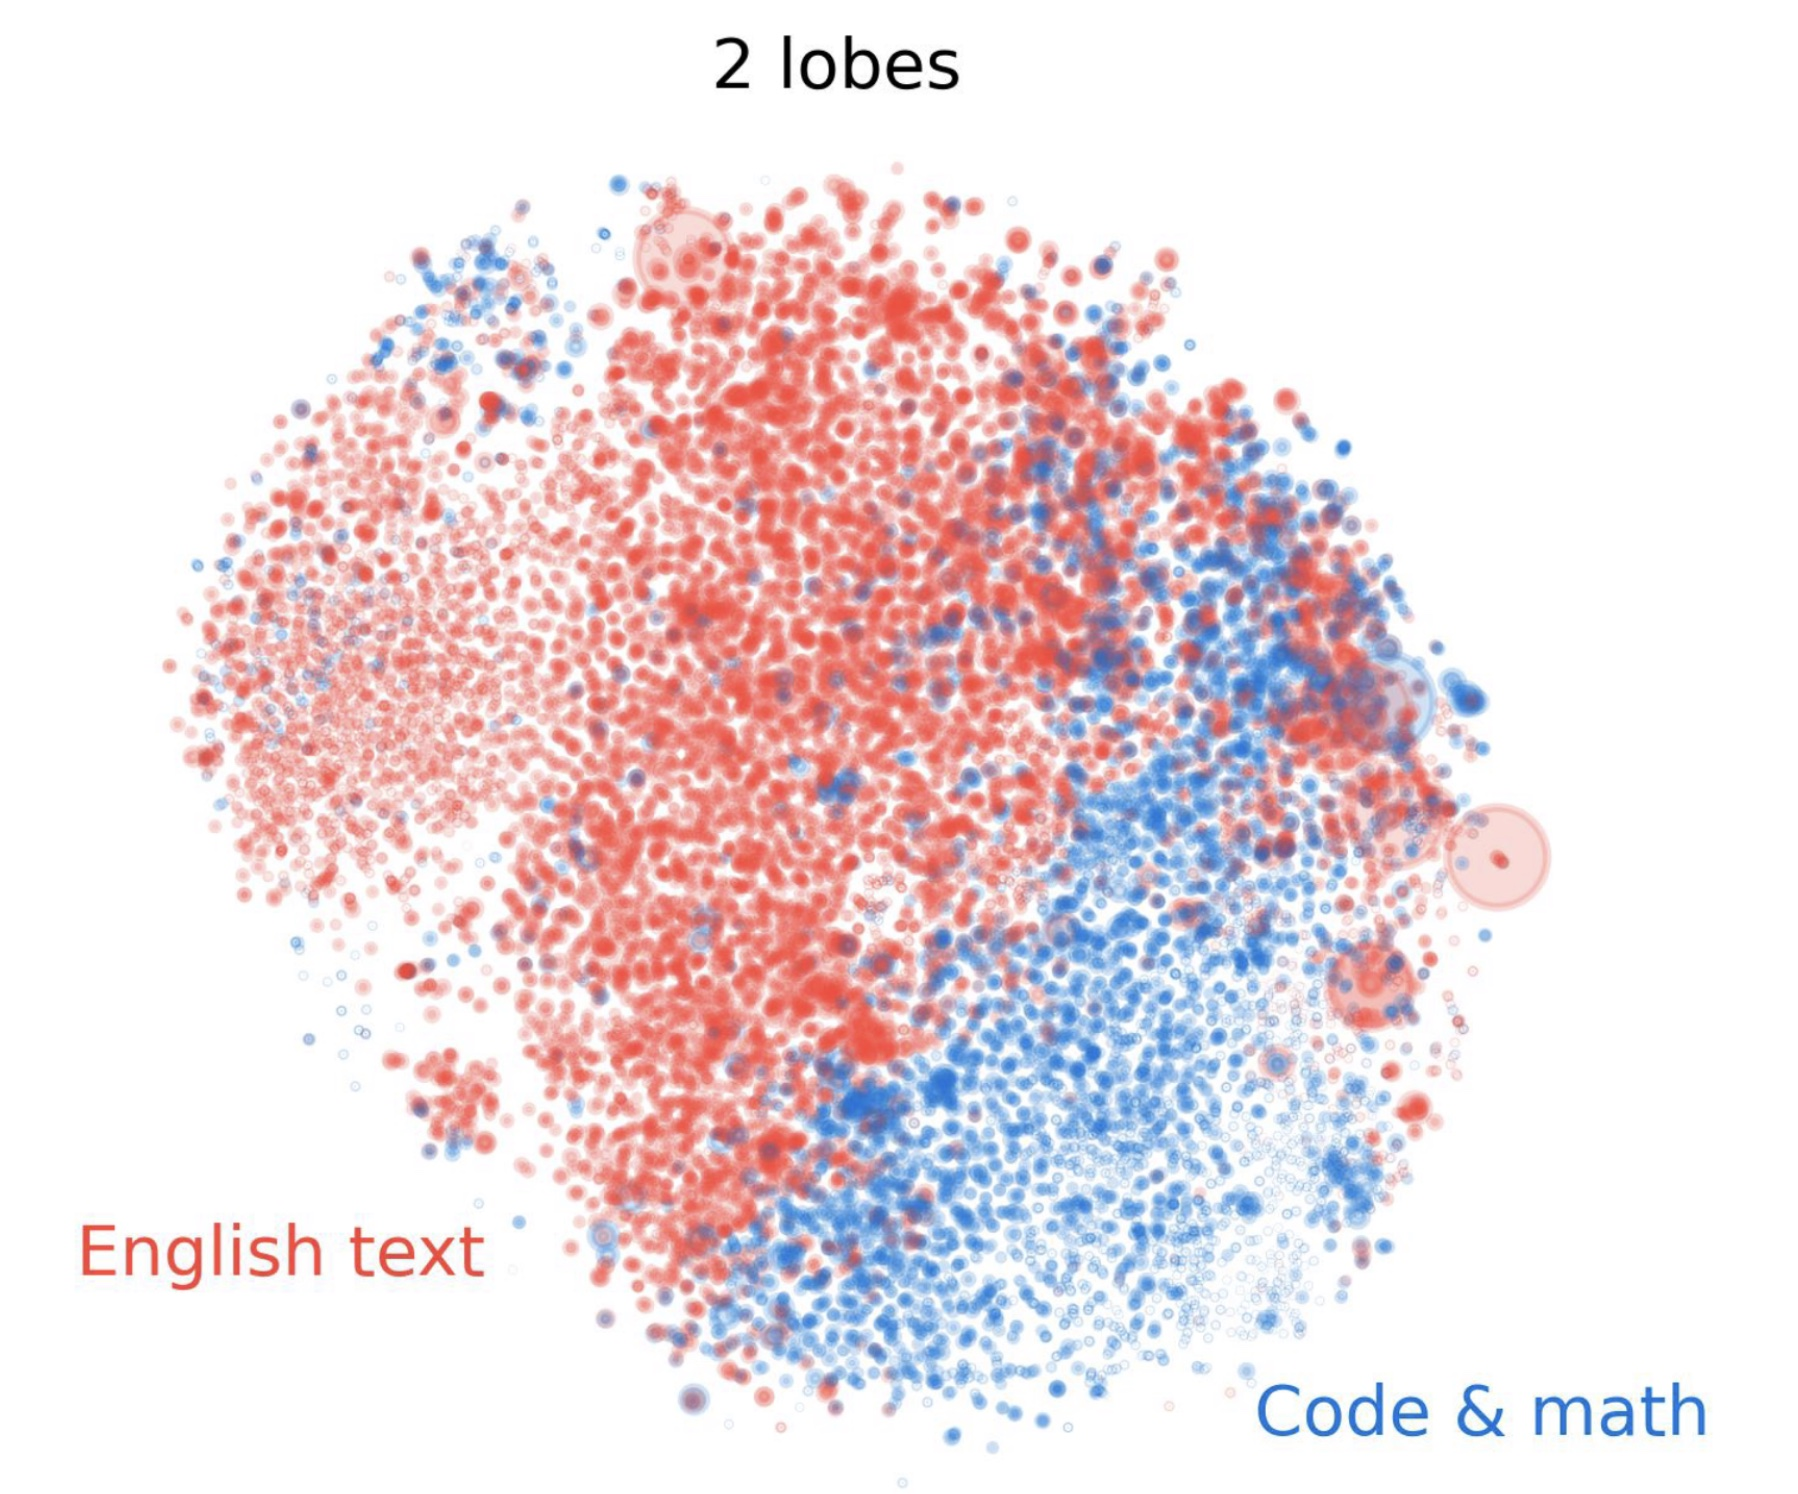
\includegraphics[width=0.5\linewidth]{figures/2-lobe-partition.jpg}}
\caption{Part of Figure 2 of~\cite{li2024Geometry}.}\label{fig:2-lobe-partition}
\end{figure}

\section{Preliminaries}
\label{sec:preliminaries}

\subsection{Sparse autoencoders}
\label{sec:sparse-autoencoders}

Given an input vector \(\mathbf{x} \in \mathbb{R}^n\), a SAE decomposes and reconstructs this vector using a
pair of encoder and decoder functions \(\left( f_{\enc}, f_{\dec} \right)\) defined by
\begin{align}
\label{eq:1}
  \mathbf{z} &= f_{\enc} \left( \mathbf{x} \right) := \sigma \left( W_{\enc} \mathbf{x} +
               \mathbf{b}_{\enc} \right), \\
  \hat{\mathbf{x}} &= f_{\dec} \left( \mathbf{z} \right) := W_{\dec} \mathbf{z} + \mathbf{b}_{\dec},
\end{align}
where \(\sigma\) is an activation function that ensures the non-negativity of linear
weights \(\mathbf{z} \in \mathbb{R}^m\). Although ordinary autoencoders tend to have \(m<n\), here we
set \(m \gg n\) because polysemanticity suggests that more features than the number of neurons are
learned by the model. When \(\mathbf{x}\) is the internal activation of a language
model, \(\mathbf{z}\) is a set of linear weights that specify how to combine columns of \(W_{\dec}\)
to reproduce \(\mathbf{x}\), and columns of \(W_{\dec}\) are directions into which the SAE
decomposes \(\mathbf{x}\), thus representing conceptual features learned by the original language
model. Sparsity of \(\mathbf{z}\) is enforced by adding a regularization term to the reconstruction
loss, and the resulting loss function for training SAEs is
\begin{equation}
\label{eq:2}
\mathcal{L} \left( W_{\enc}, W_{\dec}, \mathbf{b}_{\enc}, \mathbf{b}_{\dec} \right) = \left\| \mathbf{x} -
  \hat{\mathbf{x}} \right\|_2^2 + \lambda \left\| \mathbf{z} \right\|_0,
\end{equation}
while some implementations use an \(l_1\) penalty~\citep{cunningham2023Sparse, gao2024Scaling},
which has some disadvantages like penalizing feature magnitudes in addition to sparsity and
requiring an additional constraint on SAE parameters to enforce
sparsity~\citep{rajamanoharan2024Jumping}.

\subsection{JumpReLU SAEs}
\label{sec:jumprelu-saes}

Following \cite{lieberum2024Gemma}, this project adopts JumpReLU SAEs as they show a slight Pareto
improvement over ReLU SAEs~\citep{cunningham2023Sparse} and TopK SAEs~\citep{gao2024Scaling}. The
JumpReLU activation uses a shifted Heaviside step function parameterized by a threshold
parameter \(\bm{\theta}\), and the activation function is
\begin{equation}
\label{eq:3}
\sigma \left( \mathbf{y} \right) := \mathbf{y} \odot H \left( \mathbf{y} - \bm{\theta} \right),
\end{equation}
where \(\odot\) denotes element-wise multiplication, and \(H\) is the Heaviside step function, whose
value is \(1\) if its input is positive and \(0\) otherwise, and with a little abuse of notation,
extends to vectors. Intuitively, the JumpReLU leaves out features whose pre-activations are below
certain thresholds learned for each feature.

Note that the loss function specified by Equation~\ref{eq:2} provides no gradient signal for
training the threshold parameter \(\bm{\theta}\) because \(\bm{\theta}\) only appears within the Heaviside
step function. So this project uses straight-through-estimators (STEs; \cite{bengio2013Estimating})
to train \(\bm{\theta}\), following \cite{rajamanoharan2024Jumping} and \cite{lieberum2024Gemma}. This
introduces an additional hyperparameter, the kernel density estimator bandwidth \(\epsilon\), which
controls the quality of gradient estimates used to update \(\bm{\theta}\).

\section{Implementation}
\label{sec:implementation}

\subsection{Open-source libraries}
\label{sec:open-source-libr}

This project uses TransformerLens~\citep{nanda2022TransformerLens} to collect internal activations
of LLMs inferencing on some text. This project also uses pandas~\citep{mckinney2010Data} version
2.2.3~\citep{thepandasdevelopmentteam2024Pandasdev} and
\href{https://github.com/dask/fastparquet}{fastparquet} to save and load text data. For implementing
and training SAEs, this project uses JAX~\citep{jax2018github} and Flax~\citep{flax2020github} as
well as some libraries within their ecosystem for JAX's incredible speed and elegance compared to
PyTorch~\citep{ansel2024PyTorch}.\footnote{But TransformerLens uses PyTorch internally.} For
post-processing of learned features, like clustering, dimension reduction, and visualization, this
project uses NumPy~\citep{harris2020Array}, Scikit-learn~\citep{pedregosa2011Scikitlearn}, and
Matplotlib~\citep{hunter2007Matplotlib}. For a comprehensive list of dependencies, please refer to
the \href{https://github.com/gzqaq/aiaa-5047-project}{GitHub repository} that holds source code of
this project.

\subsection{Base LLM}
\label{sec:base-llm}

Since this project focuses on identifying partitions between different languages within the SAE
point cloud, a multilingual LLM is required. Due to my personal interest in Chinese and English, and
the outstanding Chinese capabilities of the Qwen family, this project chooses Qwen2
7B~\citep{yang2024Qwen2} from which activations are collected.\footnote{Since TransformerLens hasn't
  supported Qwen2.5, this project uses Qwen2 7B, which also surpasses Gemma 2 on Chinese tasks.}

\subsection{Dataset}
\label{sec:dataset}

\paragraph{Chinese and English text}

The best choice for text on which activations are collected is to collect from those on which the
base LLM was pretrained. However, since \cite{yang2024Qwen2} doesn't release details about training
data, alternatives are needed. Finally this project chooses Chinese and English text from a single
multilingual dataset, CulturaX~\citep{nguyen2023CulturaX}, for consistency of data quality between
these two languages.

\paragraph{Location}

Among the 28 layers of Qwen2 7B, this project chooses activations on the post MLP residual stream of
the 1st, 11st, and 21st layers (indexed from zero) based on my personal preference, since there is
not enough time and resources to train SAEs for every layer and location.

\paragraph{Amount of data}

Due to storage limitations, this project accumulates activations for approximately 10M token per
language and layer, resulting in a total of over 20 million tokens per layer for training purposes,
while \cite{lieberum2024Gemma} consumed at least 4B tokens for training SAEs of equal size
(\(m=2^{14}=16384\)). This process consumed 802GB of storage capacity. For evaluation, we collected
0.1M activations for each language and layer.

\paragraph{Preprocessing}

All collected activations are normalized by a fixed scalar to have unit mean squared norm, following
\cite{lieberum2024Gemma}. This helps more reliable transfer of hyperparameters between layers, since
norms of original activations may vary over multiple orders of magnitude. Since this project doesn't
study LLM's behavior with activations replaced by reconstructed ones, this scalar is of no later
use.

\subsection{JumpReLU SAE}
\label{sec:jumprelu-sae}

Implementation of JumpReLU SAE generally follows \cite{rajamanoharan2024Jumping} and
\cite{lieberum2024Gemma}, with a few details worth noting.

\paragraph{Straight-through-estimators}

Thanks to the flexibility of JAX's API, straight-through-estimators can be easily implemented by
registering custom backward functions of the Heaviside step function and JumpReLU activation
function using \texttt{jax.custom\_vjp}. For full Python code please refer to
\texttt{src/models/utils.py} inside the \href{https://github.com/gzqaq/aiaa-5047-project}{GitHub
  repository}.

\paragraph{Normalization of \(W_{\dec}\)'s columns}

When \(l_1\) penalty is adopted in the loss function \eqref{eq:2}, additional normalization on the
columns of \(W_{\dec}\) is required because scaling down encoder parameters and scaling up decoder
parameters accordingly could arbitrarily shrink feature magnitudes and thus the \(l_1\)
penalty~\citep{rajamanoharan2024Jumping}. Since this project adopts the \(l_0\) penalty, there is no
need for the additional normalization. However, as this project strictly follows
\cite{lieberum2024Gemma}, which always renormalizes \(W_{\dec}\) for unit-norm columns,
normalization is done after every gradient update.

\section{Results}
\label{sec:results}

Due to limitations of time and resources, this project fails to reproduce results comparable to
Figure 2 of \cite{lieberum2024Gemma}. Among SAEs trained for those three aforementioned layers, only
the one trained on activations collected at layer 21 produces satisfactory results within due time,
whereas the sparsity loss of the other two both fail to decrease to a reasonable level. Therefore,
this section will mostly focus on results produced by the SAE trained for layer 21.

\subsection{Training dynamics}
\label{sec:training-curves}

Figure~\ref{fig:curves} shows the training dynamics of these three SAEs for different
layers. Because SAEs have a much larger latent space than the activation space, it is very easy for
them to reconstruct the input perfectly, indicated by the fast drop of the reconstruction loss to
zero in the beginning. In contrast, they suffer very high sparsity loss, indicating that they use
more features than the number of neurons the original LLM has for each layer to reconstruct
activations.  During the subsequent training process, the decrease of the sparsity loss is
accompanied by a slight increase of the reconstruction loss, indicating the sparsity-fidelity
trade-off.

\begin{figure}[htbp]
\centerline{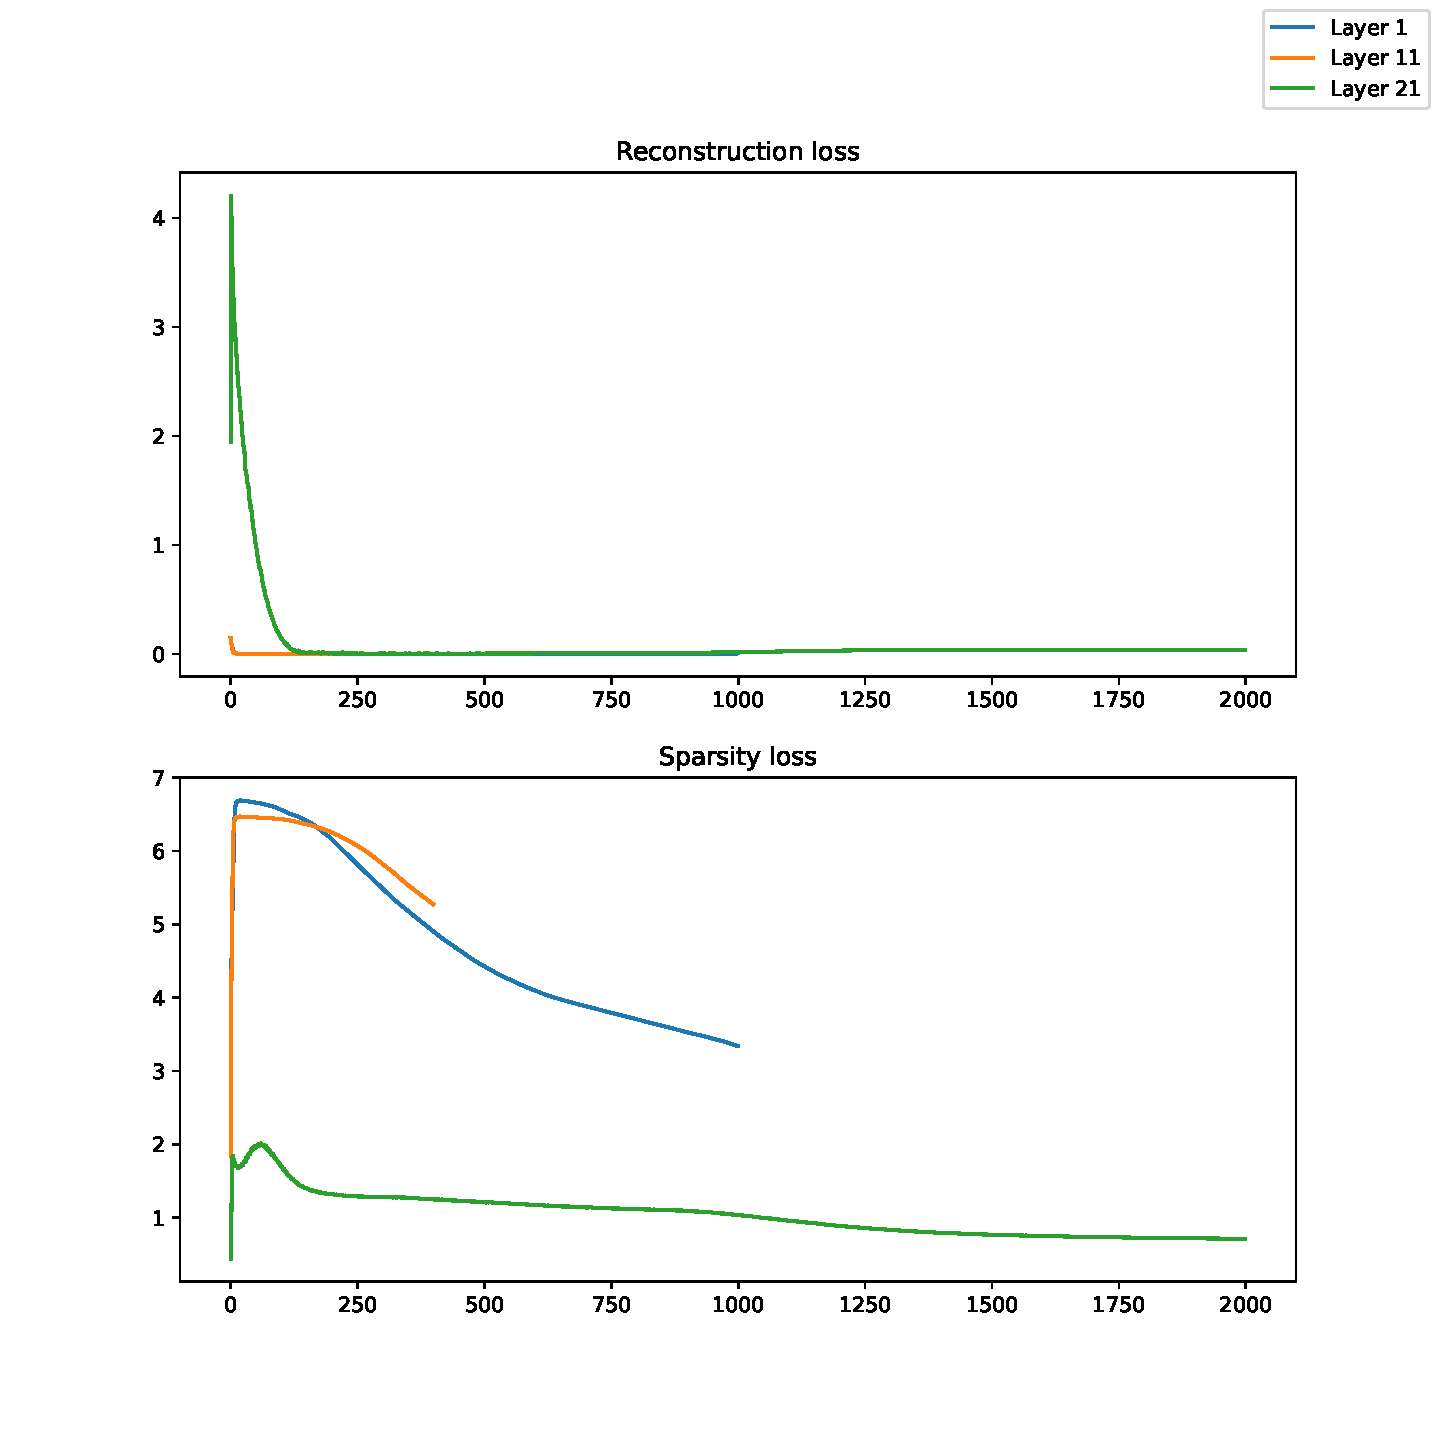
\includegraphics[width=0.7\textwidth]{figures/train-curves.pdf}}
\caption{Training curves of SAEs on three layers. The sparsity coefficient \(\lambda\) is \(0.001\), so
  the unit of the second plot's \(y\)-axis would be 1k if it represents the number of learned
  features activating for reconstruction. Training curves of SAEs for layer 1 and 11 are truncated
  due to insufficient training time.}
\label{fig:curves}
\end{figure}

\subsection{Partition of the language lobe}
\label{sec:part-lang-lobe}

This project follows Section 4 of \cite{li2024Geometry} to investigate if SAE features that are
functionally similar with respect to Chinese or English are also geometrically
similar. Specifically, a histogram of SAE feature co-occurrence is computed by feeding activations
of tokens from both Chinese and English text to the SAE and counting features as co-occurring if
they both fire within the same chunk of 256 tokens. This process is conducted on 40 chunks for each
language, selected from the 0.2M activations collected for evaluation. Given this histogram, an
affinity score is calculated between each pair of SAE features, followed by spectral clustering on
the resulting afffinity matrix.

To assess which language each lobe specializes in, for each chunk of 256 tokens, the lobe with the
highest proportion of its features firing is recorded. Thus, for each language, for each 256-token
chunk within text of that language, the lobe with the highest proportion of its SAE features firing
is recorded, and the resulting histogram of which lobes were maximally activating across each
language can be used to determine which language each lobe corresponds to.

\cite{li2024Geometry} experimented with five kinds of co-occurrence-based affinity with Phi
coefficient being the best one. Hence this project presents the main result with Phi coeffcient, but
also provides those produced by the other four measures. Note that there exist features that fire in
all chunks or don't fire at all. Since both cases are undefined behavior with respect to Phi
coeffcient, these features are filtered out.

Figure~\ref{fig:l21-phi} shows features found by the SAE for layer 21, colored according to which
lobe they belong to. Features that tend to fire together on Chinese text are seen to gather in a
small region, surrounded by those firing on English text. This indicates that LLMs do learn
different features for different languages, and features corresponding to each language are also
co-located geometrically. Figure~\ref{fig:l21-four} contains results calculated by different
affinity measures, which also show similar geometry.

\begin{figure}[htbp]
\centerline{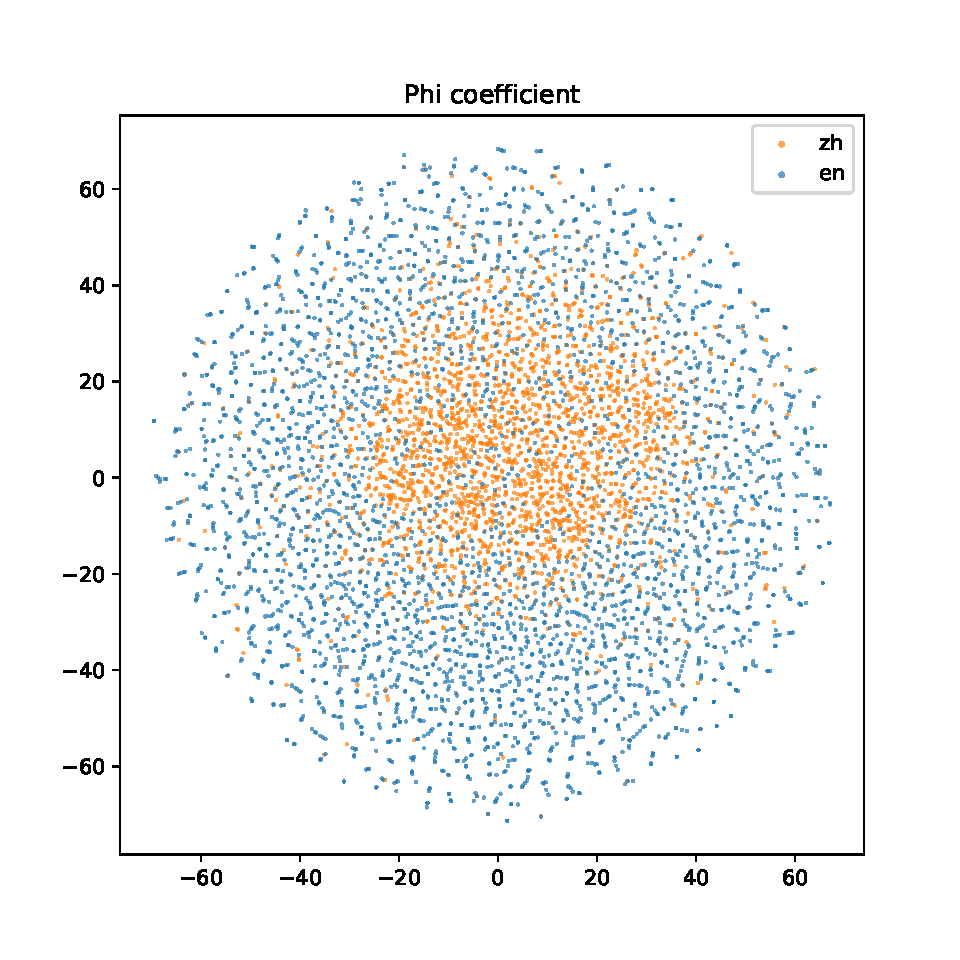
\includegraphics[width=0.75\textwidth]{figures/l21-d16384-zh-en-e2001.phi-coef.2d.pdf}}
\caption{Features of the SAE trained for layer 21 down-projected to 2D with \(t\)-SNE, color-coded
  according to the language on which they fire the most. Clusters are computed by Phi coeffcient.}
\label{fig:l21-phi}
\end{figure}

\begin{figure}[htbp]
\centerline{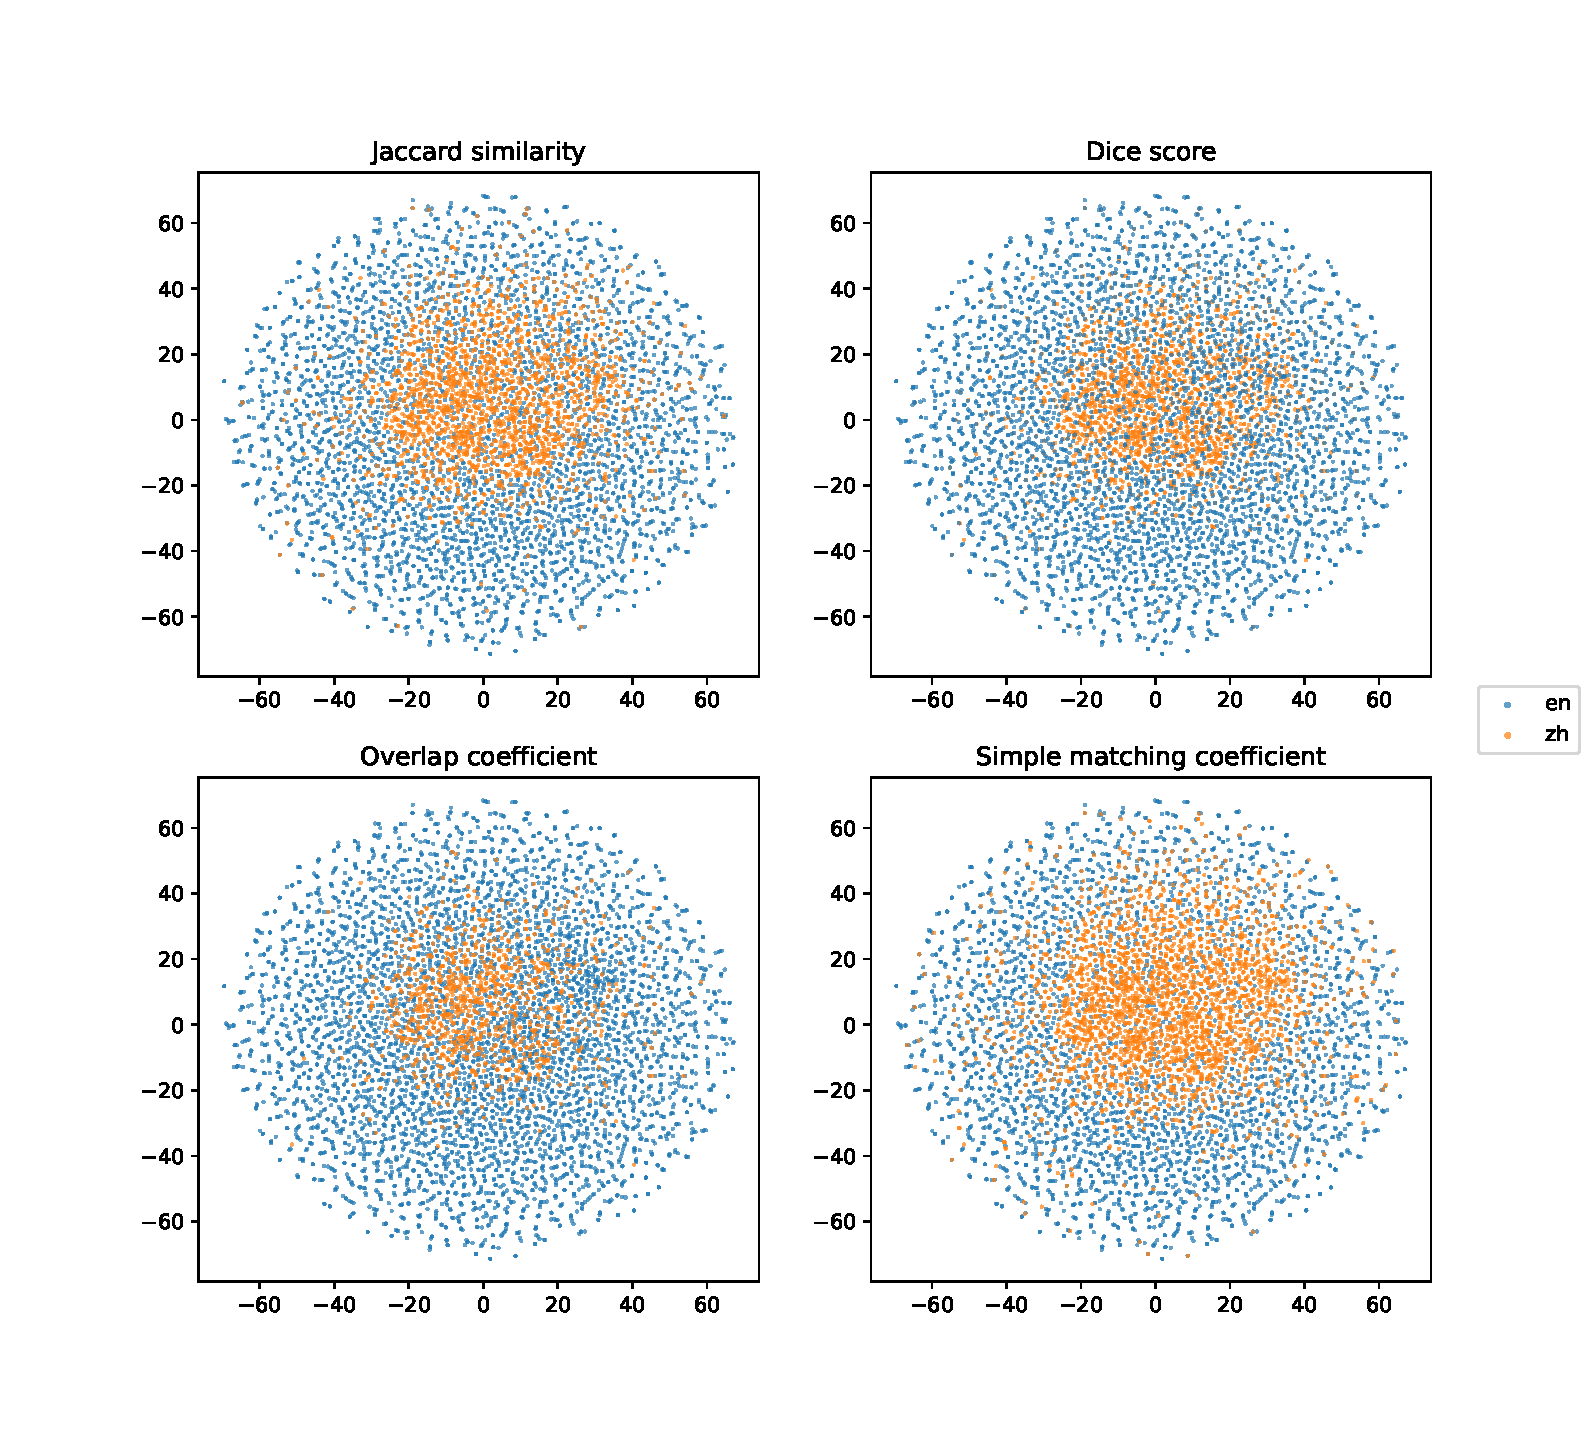
\includegraphics[width=\textwidth]{figures/l21-d16384-zh-en-e2001.four.2d.pdf}}
\caption{Features of the SAE trained for layer 21 down-projected to 2D with \(t\)-SNE, color-coded
  according to the language on which they fire the most. Clusters are computed by affinity measures
  specified by titles.}
\label{fig:l21-four}
\end{figure}

\section{Conclusion}
\label{sec:conclusion}

This project aims to investigate the functional modularity of LLMs by examining features learned by
SAEs trained within a multilingual context. Specifically, this project seeks to determine if SAE
features that activate for either Chinese or English text exhibit geometric separability, thereby
revealing potential language-specific functional modules within LLMs. Inspired by the
intermediate-scale structure identified by \cite{li2024Geometry} and employing JumpReLU SAEs trained
on activation of Qwen2 7B following setups of \cite{lieberum2024Gemma}, this project explores
partition of directions in the activation space of layer 21 that is successfully trained compared to
the other layers.

The findings demonstrate a clear geometric separation between SAE features primarily activating on
Chinese text versus those activating on English text. This separation, visualized through \(t\)-SNE
and spectral clustering based on a variety of affinity measures, suggests that LLMs learn
language-specific features that are not only functionally distinct but also spatially organized
within the activation space.

Due to the intense computational requirements for training SAEs and limited time, results presented
in this report are produced by an underfitted SAE, although certain conclusions can still be
drawn. Future work could expand this exploration to other languages, and languages within the same
language family, like Indo-European languages. As to implementation, a critical bottleneck
constraining the training speed is disk reading and data shuffling. Since Python used by this
project is still under global interpreter lock (GIL), an asynchronous version of the training
process won't parallelize data processing and gradient updating. Future work may use tools provided
by PyTorch for efficient data processing.

\bibliographystyle{plainnat}
\bibliography{refs}

\end{document}
